
\documentclass[journal]{IEEEtran}
%\usepackage{lineno}
%\linenumbers
%\usepackage{cite}
\usepackage{comment}
\ifCLASSINFOpdf
  \usepackage[pdftex]{graphicx}
  \graphicspath{pics/}
  \DeclareGraphicsExtensions{.pdf,.jpeg,.png,.jpg}
\else

\fi
\usepackage{amsmath}
\usepackage{siunitx}
\usepackage{geometry}
\usepackage{comment}
\usepackage{float}
\usepackage[caption=false]{subfig}
\usepackage[super]{nth}
\hyphenation{}

\begin{document}
\newgeometry{top=12mm, bottom=12mm, left=12mm, right=12mm}
\title{22051 - Assignment number 2}
\author{\vspace{-2mm}{\normalsize \underline{Group 3} - s194048 Erik Rame (\_ hrs), s194051 Jakob Bernhardt (\_ hrs), s194006 Steffan Kunoy (\_ hrs), \\s186083 Tjark Petersen (\_ hrs)}\vspace{-10mm}}

% make the title area
\maketitle
%\IEEEpeerreviewmaketitle

\section{How finite should it be?}

\subsection{Like a hot knife through a Butterworth}
% Erik
% Jakob
The purpose of this exercise was to construct a bandpass filter which met a set of requirements. These requirements were:
\begin{itemize}
\item Passband from 0.2 to 0.3
\item Stopbands from 0 to 0.1 and 0.4 to 1
\item Ripples are OK if they don't exceed 2 dB
\item The stopband attenuation should be at least -100 dB
\end{itemize}

It was decided to make a Butterworth bandpass filter. MATLAB has a built-in function called 'butter' which returns the transfer function of a Butterworth filter of the specified type, order and cutoff frequency. 
\newline
The requirements meant that we constructed a bandpass Butterworth filter using a higher and lower cutoff frequency of 0.2 and 0.3 respectively. The order was determined by testing the function with different values, and choosing the lowest order where the stopband attenuation was at least -100 dB. The resulting magnitude and phase response of the 12th order Butterworth bandpass filter can be seen in figure \ref{fig:butterband}.

\begin{figure} [H]
    \centering
    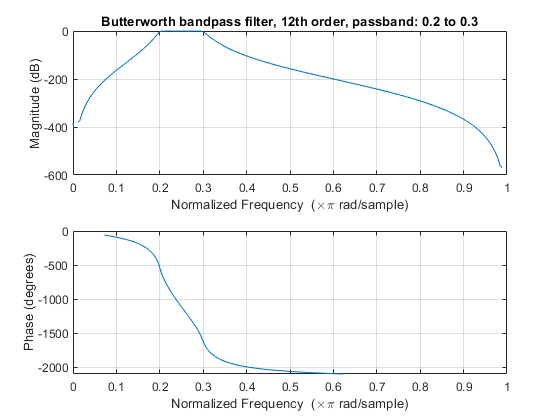
\includegraphics[width=\linewidth]{assignment_02/plots/butterbandfreq.png}
    \caption{Frequency and phase response of a Butterworth bandpass filter that lives up to the given specifications.}
    \label{fig:butterband}
\end{figure}

The next task was to compute and plot the impulse response (figure xx) and the pole-zero plot in the z-plane (figure xx). 
% insert impulse response and pole-zero plot

Using the computed impulse response, we were asked to find the effective length of the impulse response, which is the length (in samples) at which the impulse response decays below 10\% of its maximum. This was done in practice by ...
Using the computed impulse response, we were asked to find the effective length of the impulse response, which is the length (in samples) at which the impulse response decays below 10\% of its maximum. This was done in practice by ...

\subsection{Shorter and shorter}
% Steffan
For this exercise we were tasked with designing an \textit{ideal} FIR lowpass filter based on the following specifications: 
\begin{itemize}
    \item Pass-band from 0 to 5 kHz with gain of 0 dB. 
    \item Cut-off frequency at one-third the normalized frequency. 
    \item Impulse response is 601 samples long. 
\end{itemize}
From these specifications we can argue that the sampling frequency should be 30 kHz, as the Nyquist frequency would then be 15 kHz, which would correspond to three times the cut-off frequency of 5 kHz. A frequency response of the proposed filter is shown in Figure \ref{fig:freq_resp_lowpass}. We see that the idealized filter has an infinitely steep roll-off at the break frequency and also zero phase shift, meaning no time delays. Applying the inverse Fourier transform yields the time-domain impulse response shown in Figure \ref{fig:imp_resp_lowpass}. The impulse response can be seen to be acausal and periodic centered around 

\begin{figure}
    \centering
    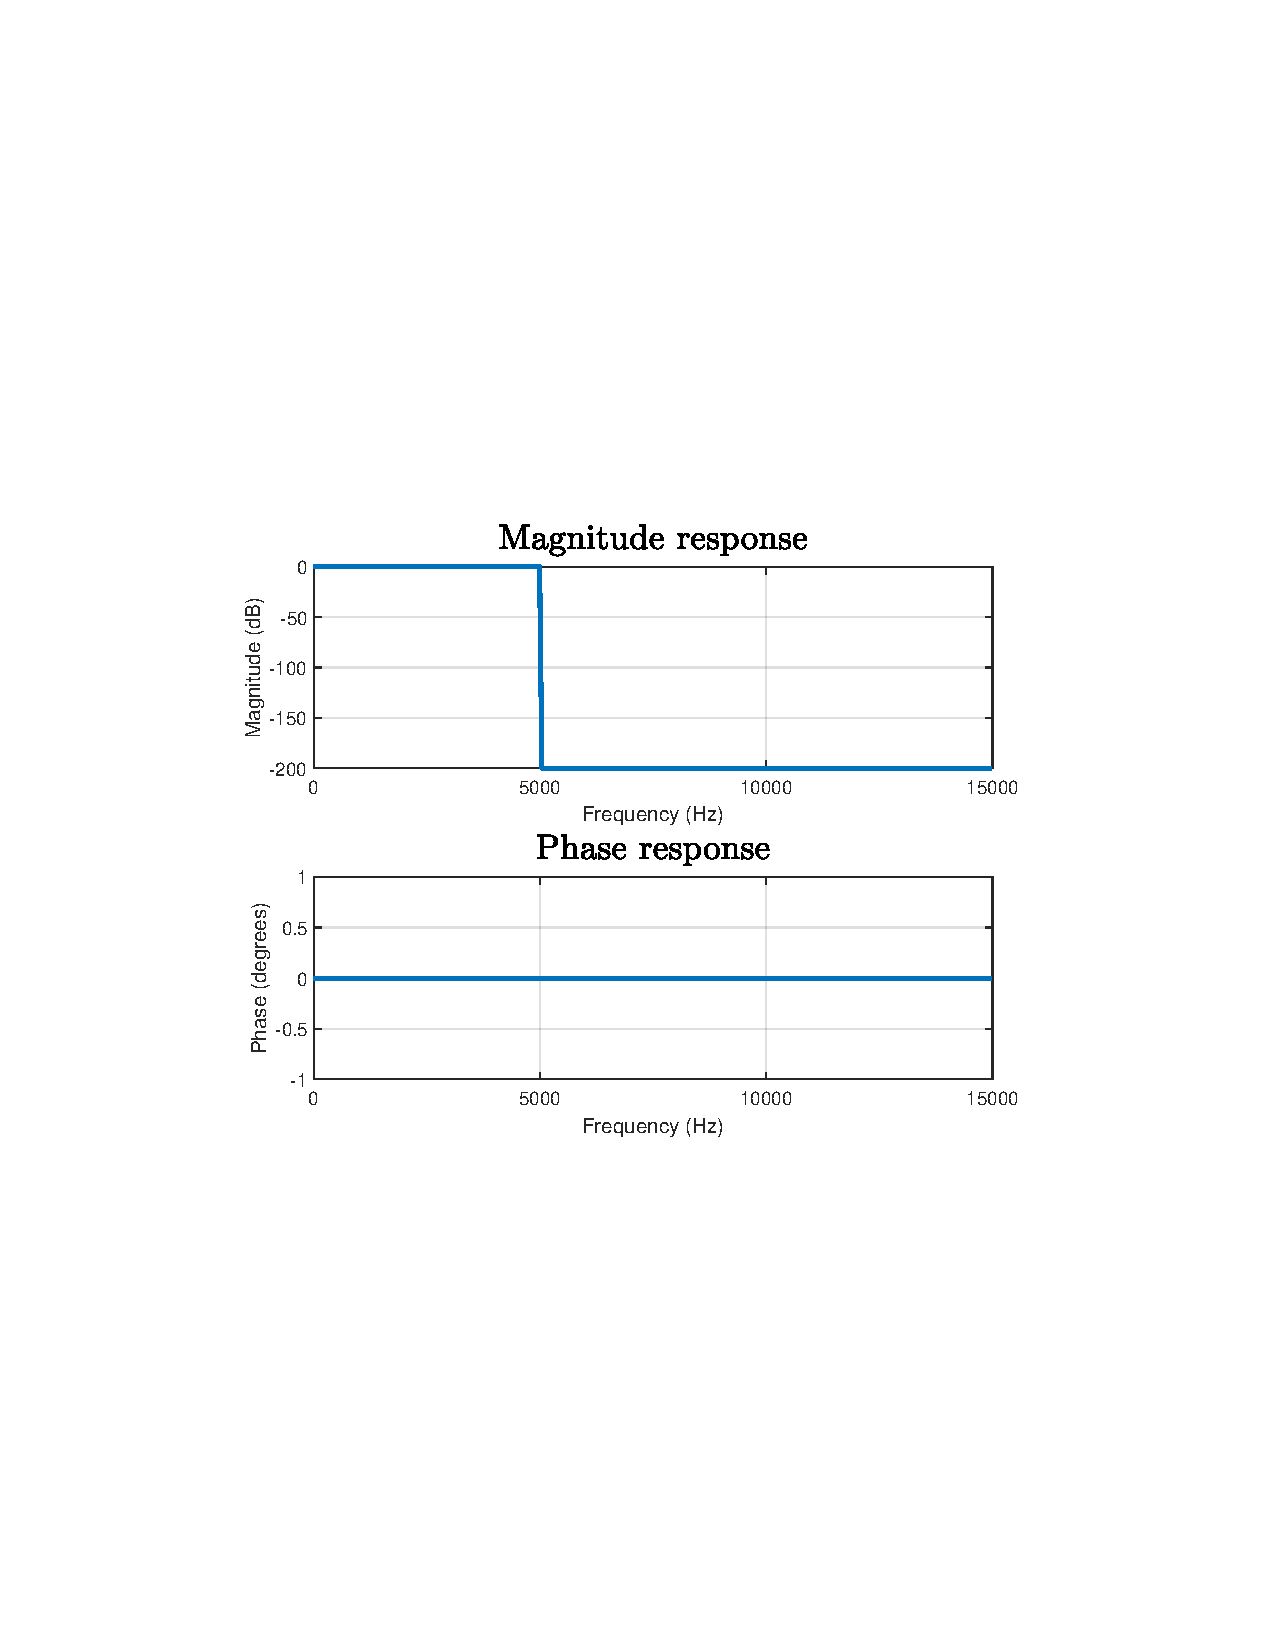
\includegraphics[width=\columnwidth,clip]{assignment_02/plots/freq_resp_lowpass_fir.pdf}
    \caption{Frequency response of the idealized low-pass filter.}
    \label{fig:freq_resp_lowpass}
\end{figure}

\begin{figure}
    \centering
    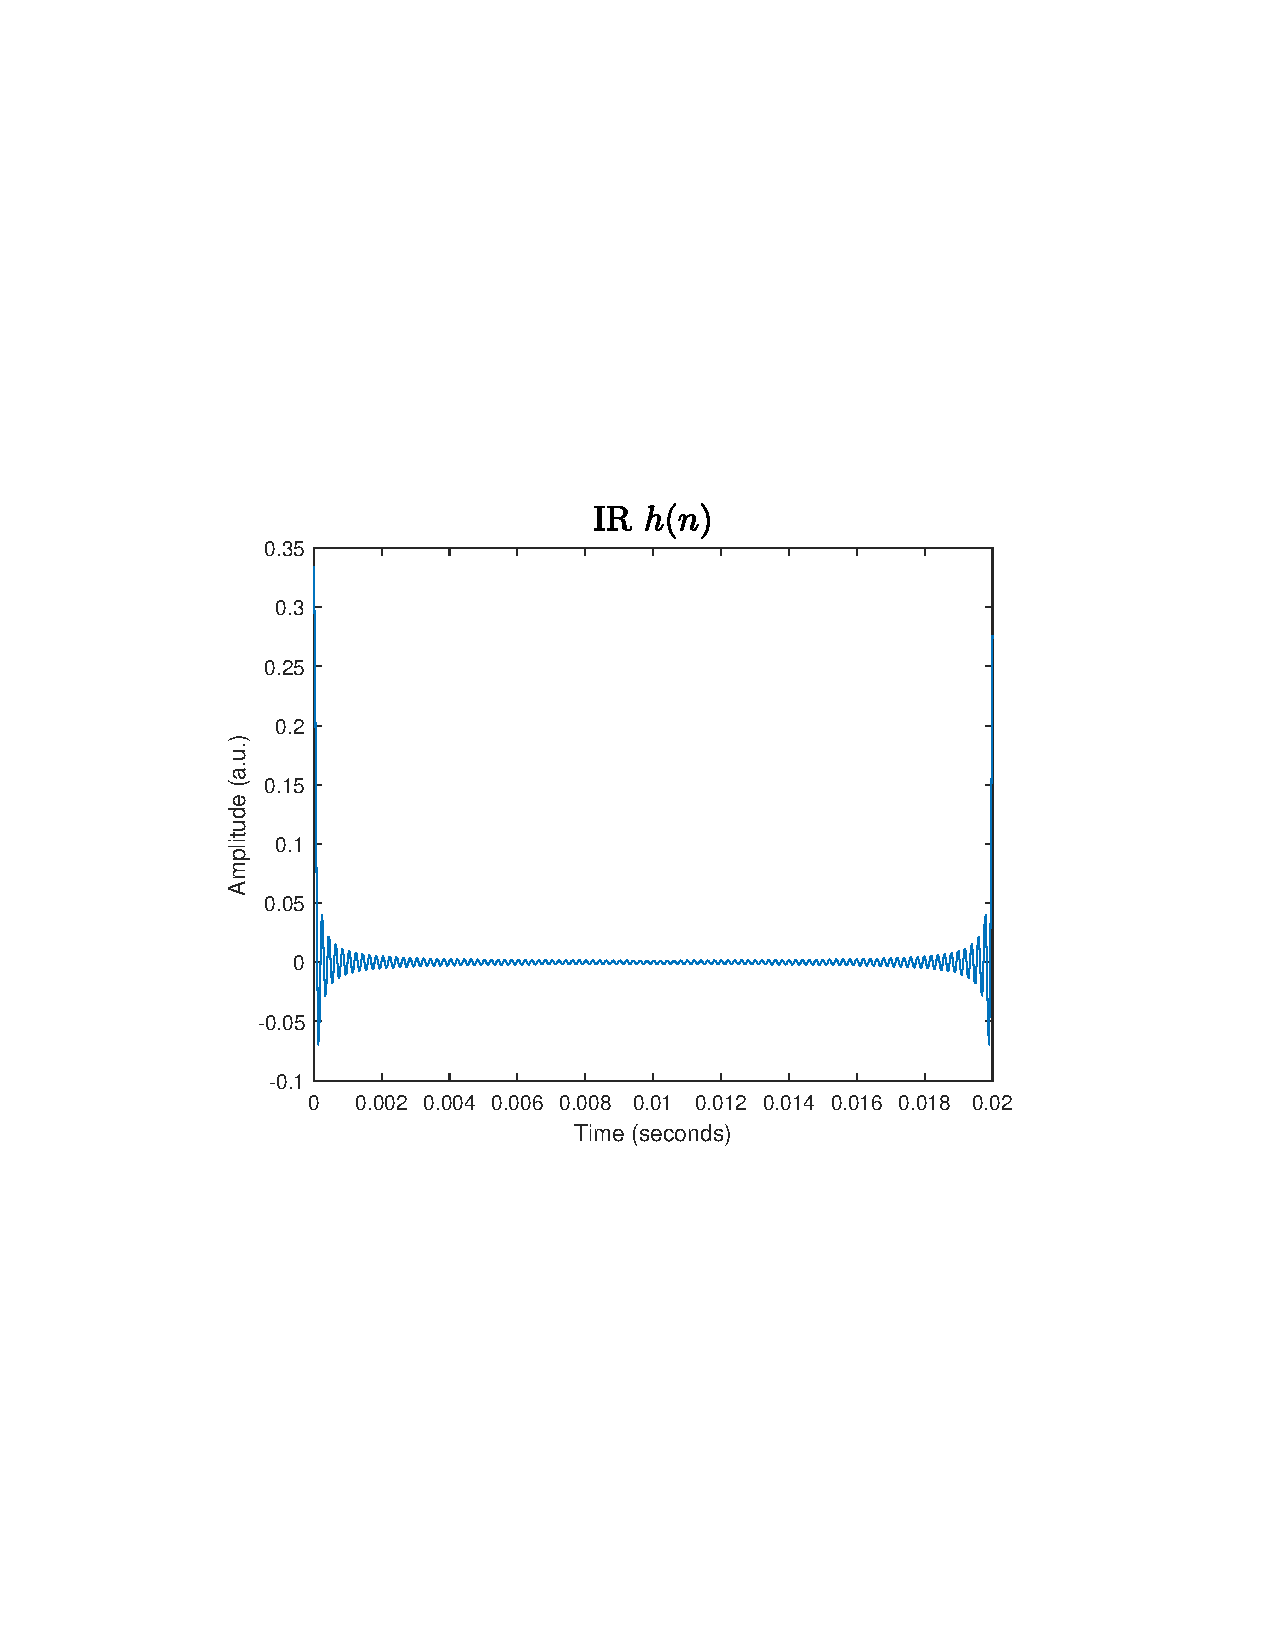
\includegraphics[width=\columnwidth,clip]{assignment_02/plots/impulse_resp_lowpass_fir.pdf}
    \caption{Impulse response of ideal lowpass filter.}
    \label{fig:imp_resp_lowpass}
\end{figure}


\newpage

\section{An equalizer - without buttons}
\subsection{Bass and treble}
% Tjark

One application of FIR filters lies in the domain of digital audio processing where the finite nature of the filter response corresponds to a known and limit number of computations per output sample which is impossible to have when using an IIR filter. In the following section, the use of an FIR band-pass filter as an equalizer is investigated. The filter will be obtained using the frequency domain equivalence method for FIR filters.

The bandpass filter used as an equalizer can be characterized by four parameters: the two normalized cut-off frequencies contained in the set $\omega_c$, the pass-band gain $G_p$ and the IR length $L$. Here the term \textit{pass-band gain} should not be taken strictly, since a negative pass-band gain is a legal parameter.

Using this set of parameters, an ideal bandpass filter can be constructed in the frequency domain. For this all frequencies outside of the pass-band are set to 0 dB while all frequencies inside of the pass-band itself are set to $G_p$. An example of an obtained ideal frequency response is shown in Fig. \ref{fig:eq}.

\begin{figure}
    \centering
    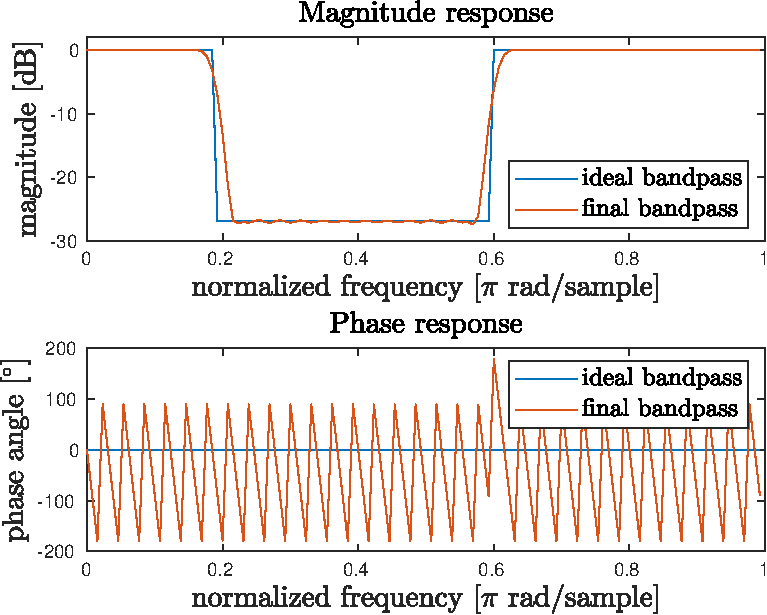
\includegraphics[width=\columnwidth]{assignment_02/plots/equalizer.pdf}
    \caption{The frequency response for the ideal and final equalizer filter using the cut-off frequencies $\omega_c=\{0.2,0.6\}$, a pass-band gain of $G_p=-27$ dB and a filter length of $L=260$.}
    \label{fig:eq}
\end{figure}
\begin{figure}
    \centering
    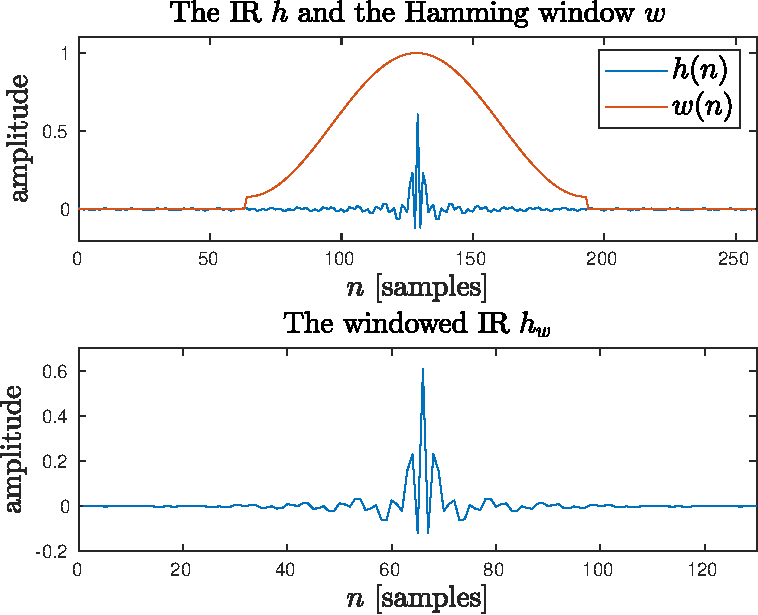
\includegraphics[width=\columnwidth]{assignment_02/plots/equalizer_ir.pdf}
    \caption{(top) The impulse response $h(n)$ for the ideal band-pass filter and a Hamming window $w(n)$ cutting of 50\% of the IR. (bottom) The impulse response for the final equalizer filter. Both use cut-off frequencies of $\omega_c=\{0.2,0.6\}$, pass-band gains of $G_p=-27$ dB and filter lengths of $L=260$.}
    \label{fig:eq_ir}
\end{figure}

The frequency response is then sampled to obtain a discrete spectrum which in turn is transferred to the time domain using the inverse Fourier transform. Since the spectrum resembles a $rect$ function, the resulting impulse response $h$ in the time domain is a $sinc$ function. The IR is periodic due to the periodicity of a digital spectrum. We consider one period which has the peak of the $sinc$ function centered at $n=0$. This IR is not causal since it starts to rise before $n=0$. In order to make it causal, the IR is shifted by half a period in time. The result can be seen in Fig. \ref{fig:eq_ir}. 

It can be observed, that the IR is close to zero for a large part of one period. We can therefore shorten the IR using windowing and thus get a computationally less demanding filter without compromising the frequency response significantly. For this, a Hamming window $w$ is used which can be seen in Fig. \ref{fig:eq_ir}. The window is centered around the $sinc$ function's peak. The resulting IR $h_w$, where the window has been applied, is shown at the bottom of Fig. \ref{fig:eq_ir}.

For an FIR filter, $a = \{1\}$ while the $b$ coefficients are equal to the IR itself. We can thus find our final equalizer filter coefficients in the windowed impulse response $h_w$. The spectrum of the resulting filter can be compared to the ideal starting point in Fig. \ref{fig:eq}. Due to windowing, we have introduced some oscillations and a generally wider transition band around the cut-off frequencies. The most distinctive feature though is the phase response. By making our IR causal, a phase delay had to be introduced for certain frequencies. Since our IR is finite and point symmetric, the phase response is linear nevertheless, which makes it phase distortion free. This of course is a requirement for any audio application. 

The accompanying Matlab live script makes it possible to apply the filter to music and use it as a basic equalizer. The resulting audio shows the expected behavior when for instance low frequencies are blocked or amplified. 

To make the equalizer control more interactive, a block processing implementation was attempted using a combination of the \texttt{sound} and \texttt{pause} as well as the stopwatch functions in Matlab. Since the impulse response can be kept very short, there is only very little overlap between two blocks and the overlap was therefore ignored. The whole goal of the implementation though, to make the equalizer more interactive, was defeated by the fact that Matlab's execution engine does not recognize changes in the script variables during execution.

To conclude, the FIR filter approximation of an ideal band-pass filter using the frequency domain equivalence method for FIR filters seems to yield very satisfactory results while keeping the computational cost at a minimum. It seems therefore especially suitable for real time audio processing applications.




\end{document}


